\section{Single Inverted Pendulum Model}
The simple inverted pendulum is the most basic model used to simplify humanoids' body. The basis of the pendulum are a mass $m$ linked to a pivot point $0$ by means of a massless link of longitude $l$ as in Figure \ref{fig:pendulo_inv}.

The mass $m$ represents the total mass of the modelled system, a humanoid robot in this case, located at its Centre of Mass (CoM), and the longitude $l$ is the distance between the pivot point to the CoM. Its dynamical model in a planar, for example XZ case, is expressed by the equation \eqref{eq:pendulo}, if gravitational force is considered the only force acting in the system.

\begin{figure}
\centering
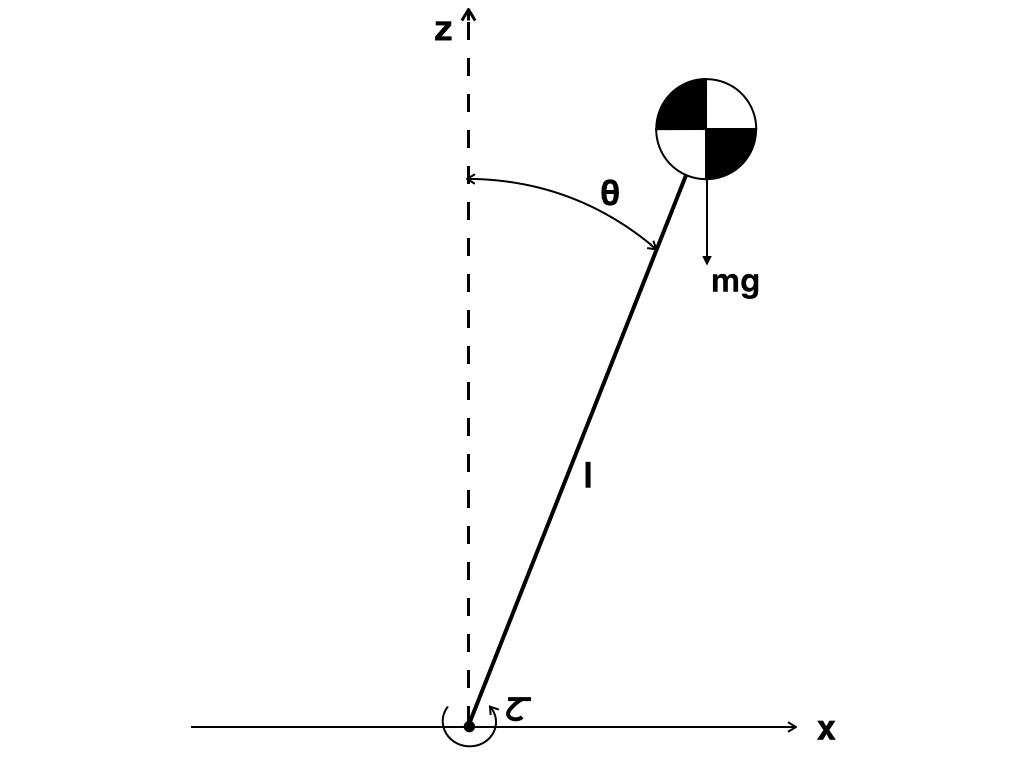
\includegraphics[scale=0.25]{pendulo_inv.png}
\caption{Single inverted pendulum.}
\label{fig:pendulo_inv}
\end{figure}

\begin{equation}
\tau_0 = ml^2 \ddot{\theta} - mgl\sin\theta
\label{eq:pendulo}
\end{equation}

where $\tau_0$ is the torque generated by the ankle joint, $\theta$ its angular position, $\ddot{\theta}$ its angular acceleration and $l$, the distance between the joint and the CoM. For simplification of a control task, let us make a linearization of nonlinear differential equations, taking the aproximation that perturbations are small enough to consider  $\sin\theta = \theta$. It is not defined how small these angles have to be in practice to apply the linearization assumptions, but in this case it is assume that $\theta \leq 5º$ Then, equation \eqref{eq:pendulo} changes to linearized equation \eqref{eq:pendulo2}
\begin{equation}
\tau_0 = ml^2 \ddot{\theta} - mgl\theta
\label{eq:pendulo2}
\end{equation}

The main complexity of this model is the fact that equation \eqref{eq:pendulo2} does not give the possibility of controlling the ZMP by angular position of the ankle joint. To overcome this problem, the inverted pendulum model can be slightly modified. The link of the pendulum which connects the ankle joint to the concentrated mass (CoM) is generally assumed to be rigid. However, in the real humanoid mechanism it is flexible because the leg length is relatively long and the mechanical structure suffers form flexibility and small backlashes. Because of this compliance, the humanoid robot exhibits the characteristics of a lightly damped structure \cite{Kim2004}. For example, in a static case when the ankle joint is under position control, a pushing external force can easily excite an oscillation. This oscillation exists even when the position error in every joint is zero. This phenomenon is prevalent in the fast dynamical gait; therefore it is very imortant to implement a control mechanism allowing ZMP fast correction considering the stiffness of the humanoid robot links. The most suitable model in this case will be a single mass inverted pendulum with compliant joint as shown in Figure \ref{fig:pendulo_elast}, where $u$ denotes the ankle joint reference angle and $\theta$ denotes the actual inclined angle produced by the compliance of the mechanical structure of the humanoid, $k$ denotes the stiffness of the leg and $\tau_0$ is the torque produced by the motor of the ankle joint to place the inverted pendulum into the desired angular position. Then, the torque $\tau_0$ should be expressed as:

\begin{equation}
\tau_0 = k(\theta - u)
\label{eq:pendulo3}
\end{equation}

\begin{figure}
\centering
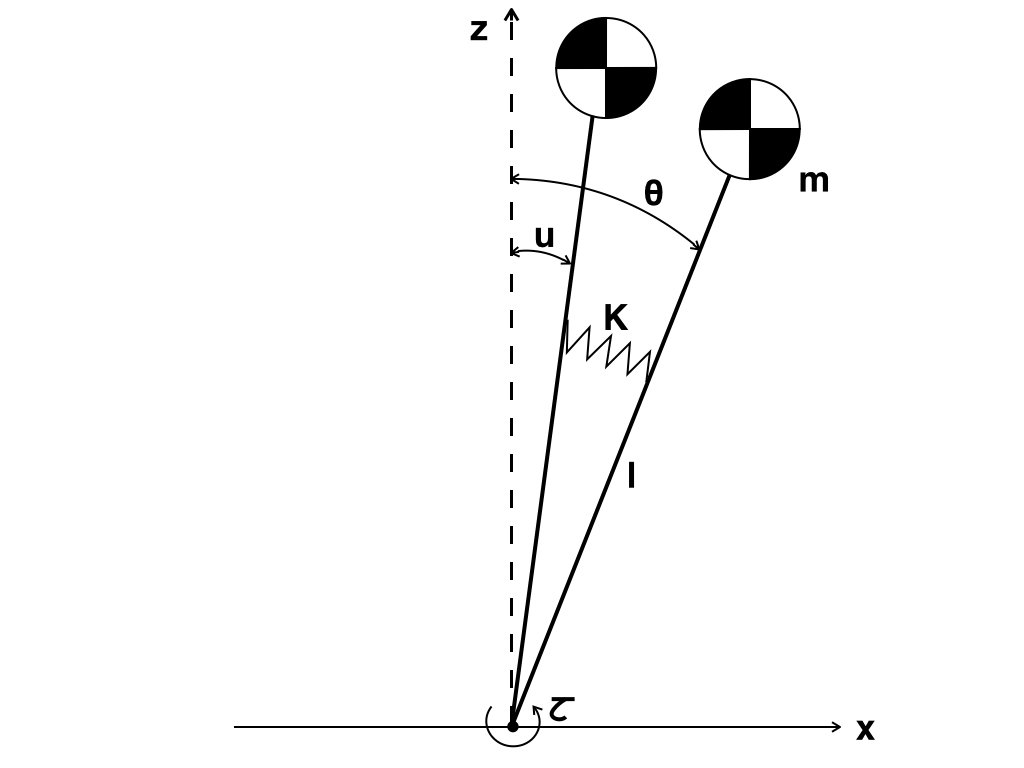
\includegraphics[scale=0.25]{pendulo_elast.png}
\caption{Single inverted pendulum with compliant joint.}
\label{fig:pendulo_elast}
\end{figure}

Taking the Laplace transform of equation \ref{eq:pendulo2}, it is obtained: 
\begin{equation}
T(s) = mgl\theta(s)- ml^2s^2\theta(s) 
\label{eq:par}
\end{equation}

The Laplace transform of equation \eqref{eq:pendulo3} is:
\begin{equation}
T(s) = k(\theta(s) - U(s))
\label{eq:par2}
\end{equation}

Reflecting $\theta(s)$ from equation \eqref{eq:par2} and placing it into the equation \eqref{eq:par} and simplifying, the transfer function is obtained:
\begin{equation}
\frac{T(s)}{U(s)} = k \frac{-s^2+(\beta - \alpha)}{s^2 + \alpha}
\label{eq:TFpar}
\end{equation}

where:
\begin{equation}
\alpha = \frac{k-mgl}{ml^2}
\end{equation}
\begin{equation}
\beta = \frac{k}{ml^2}
\end{equation}

On the other hand, from equation \textcolor{red}{[REF ECUACION zmp]} relating the moment produced by the ground reaction force around $y$ axis with $x$ ZMP direction (the planar XZ case of the inverted pendulum is considered) we can get:
\begin{equation}
\tau_y = -mgx_{ZMP} = - F_z x_{ZMP}
\label{eq:zmp}
\end{equation} 

and then the Laplace transform of the equation \eqref{eq:zmp} is:
\begin{equation}
\tau_y(s) = - F_z x_{ZMP}(s)
\label{eq:TFzmp}
\end{equation}

For the static equilibrium of the system, the moment generated y the motor of the ankle join should compensate the moment produced by the ground reaction force:
\begin{equation}
\tau_0 = \tau_y
\end{equation}

The relation between $\tau_y$ and $x_{ZMP}$ is lineal, therefore, placing \eqref{eq:TFzmp} into \eqref{eq:TFpar} we get the following transfer function relating ZMP to ankle joint position: 
\begin{equation}
\frac{x_{ZMP}(s)}{U(s)} = - k_1 \frac{-s^2+(\beta - \alpha)}{s^2 + \alpha}
\end{equation}

where $k_1 = \frac{k}{mg}$.

In the equation \eqref{eq:TFpar} $x_{ZMP}(s)$ is the output and $U(s)$ is the input of the system. It allows for the ZMP of the humanoid robot to be contolled by the position of its ankle joint. 

The state space representation of the dynamical system in the standard form is:
\begin{equation}
\mathbf{\dot{x}} = \mathbf{A}\textbf{x} + \mathbf{B}u
\label{eq:ss1}
\end{equation}

\begin{equation}
y = \mathbf{C}\textbf{x} + Du
\label{eq:ss2}
\end{equation}

where $\mathbf{x}$ is a state ($n$-vector), $y$ is the output (escalar), $u$ - control (scalar), $\mathbf{A}$ - $n \times n$ constant  matrix, $\mathbf{B}$ - $n \times 1$ constant matrix, $\mathbf{C}$ - $1 \times n$ constant matrix and $D$ a scalar.

To obtain the state representation of the inverted pendulum system let us define state variables $x_1$ and $x_2$ by:
\begin{equation}
x_1 = \theta
\label{eq:x1}
\end{equation}
\begin{equation}
x_2 = \dot{x_1} = \dot{\theta}
\label{eq:x2}
\end{equation} 

where angle $\theta$ denotes the rotation of the pendulum about the ankle and $\dot{\theta}$ its angular velocity. We consider the ZMP as the output of the system, then $y = x_{ZMP}$ in the XZ plane case. From the definition of state space equations \eqref{eq:ss1} - \eqref{eq:x2} and the linearized equations of the inverted pendulum motions \eqref{eq:pendulo2} and \eqref{eq:pendulo3} we obtain the state space representation of the system:
\begin{equation}
\begin{bmatrix}
\dot{x_1} \\
\dot{x_2}
\end{bmatrix} 
= 
\begin{bmatrix}
0 & 1 \\
-\alpha & 0
\end{bmatrix}
\begin{bmatrix}
x_1 \\
x_2
\end{bmatrix}
+
\begin{bmatrix}
0 \\
1
\end{bmatrix}
u
\label{eq:state_space}
\end{equation}
\begin{equation}
y = \begin{bmatrix}
-k_1\beta & 0 
\end{bmatrix}
\begin{bmatrix}
x_1 \\
x_2
\end{bmatrix}
+ \begin{bmatrix}
k_1
\end{bmatrix}
u
\label{eq:state_space_out}
\end{equation}
